\documentclass{beamer}
% Use DS9 global theme (includes pgfplots for visualization)
\usepackage{../../../shared/templates/ds9_theme}

% Title page configuration
\title[Relational Logic and Control Flow]{CS12 CH:5.3 - 5.5}
\subtitle{Relational Expressions \& The if/else Statement}
\author[Mr. Gullo]{Mr. Gullo}
\date[Sep 23]{September 23rd, 2025}

\begin{document}

\frame{\titlepage}

\begin{frame}
\frametitle{Learning Objectives}
\framesubtitle{From Sections 5.3 - 5.5}
By the end of this lesson, you will be able to:
\begin{itemize}
    \item Use relational operators to compare values and form boolean expressions.
    \item Implement conditional logic using \texttt{if} and \texttt{if/else} statements to control program flow.
    \item Identify and correct the common programming error of using assignment (\texttt{=}) instead of comparison (\texttt{==}).
    \item Understand the pitfalls of comparing floating-point numbers for exact equality.
    \item Combine multiple conditions using logical operators (\texttt{\&\&}, \texttt{||}).
\end{itemize}
\end{frame}

\section{Relational Operators and Conditional Logic}

\begin{frame}
\frametitle{Relational Operators}
\framesubtitle{The Building Blocks of Decisions}
Relational operators compare two values and evaluate to a boolean result: \texttt{true} or \texttt{false}.

\begin{columns}[T]
    \begin{column}{0.5\textwidth}
        \begin{itemize}
            \item \texttt{==} \quad Equal to
            \item \texttt{!=} \quad Not equal to
            \item \texttt{>}  \quad Greater than
        \end{itemize}
    \end{column}
    \begin{column}{0.5\textwidth}
        \begin{itemize}
            \item \texttt{<}  \quad Less than
            \item \texttt{>=} \quad Greater than or equal to
            \item \texttt{<=} \quad Less than or equal to
        \end{itemize}
    \end{column}
\end{columns}

\pause

These expressions form the \alert{conditions} that control our \texttt{if} statements.
\end{frame}

\begin{frame}[fragile]
\frametitle{The \texttt{if} and \texttt{if/else} Statements}
\framesubtitle{Controlling Program Flow}

The \texttt{if} statement executes a block of code only if its condition is \texttt{true}.

\begin{minted}[fontsize=\small]{cpp}
int someNumber = 99;

if (someNumber % 2 == 0) {
    cout << "The number is even\n";
}
\end{minted}

\pause
The \texttt{else} block provides an alternative path for when the condition is \texttt{false}.

\begin{minted}[fontsize=\small]{cpp}
if (someNumber % 2 == 0) {
    cout << "The number is even\n";
} else {
    cout << "The number is odd\n";
}
\end{minted}
\end{frame}

\begin{frame}
\frametitle{Concept Visualization: Context}
\framesubtitle{How \texttt{if/else} Controls Program Flow}
An \texttt{if/else} statement creates a branch, or a fork, in the path of execution.

\begin{itemize}
    \item The program evaluates a \alert{condition}.
    \item Based on the result (\texttt{true} or \texttt{false}), it chooses one of two paths.
    \item After the chosen path is executed, the paths merge, and the program continues sequentially.
\end{itemize}

The next slide shows a flowchart of this process.
\end{frame}

\begin{frame}
\frametitle{Concept Visualization: \texttt{if/else} Flowchart}
\begin{figure}
    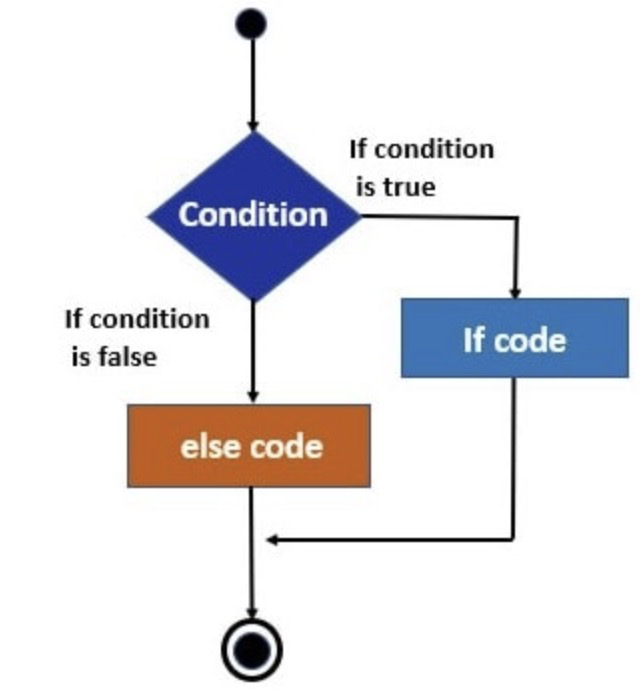
\includegraphics[width=0.5\linewidth]{cs12-if-else-flowchart.png}
\end{figure}
\end{frame}

\section{Live Demos \& Common Pitfalls}

\begin{frame}[fragile]
\frametitle{Demo: \texttt{if/else} in Action}
\framesubtitle{File: \texttt{05e\_ifElseIntro.cpp}}
This program demonstrates a complete \texttt{if/else} structure that responds to user input.

\begin{minted}[fontsize=\scriptsize, frame=lines, linenos]{cpp}
#include <iostream>
using namespace std;

int main()
{
   int inputNumber;

   cout << "Please enter an integer: ";
   cin >> inputNumber;

   if(inputNumber % 2 == 0)
      cout << "The number you entered is even\n";
   else
      cout << "The number you entered is odd\n";

   return 0;
}
\end{minted}
\end{frame}

\begin{frame}
\frametitle{Common Pitfall: Assignment vs. Comparison}
\framesubtitle{A very common and subtle bug!}

A frequent error is using the assignment operator (\texttt{=}) where the comparison operator (\texttt{==}) is intended.

\begin{itemize}
    \item \texttt{x == 13} asks the question: "Is the value of x equal to 13?" It evaluates to \texttt{true} or \texttt{false}.
    \pause
    \item \texttt{x = 13} is a command: "Assign the value 13 to the variable x." This expression itself evaluates to the assigned value, which is \texttt{13}.
\end{itemize}

In C++, any non-zero number is treated as \texttt{true} in a condition, so \texttt{if (x = 13)} will \alert{always} be true!
\end{frame}

\begin{frame}[fragile]
\frametitle{Assignment vs. Comparison: Code Example}
This code will not behave as you might expect. The `if` condition contains an assignment.

\begin{minted}[fontsize=\small]{cpp}
int x = 50;

if (x = 13) // WARNING: This is an assignment!
    cout << "Some text\n";
else
    cout << "Some other text\n";

cout << "Final value of x: " << x << endl;
\end{minted}
\pause
\vfill
\textbf{Output:}
\begin{verbatim}
Some text
Final value of x: 13
\end{verbatim}
The condition assigned \texttt{13} to \texttt{x}, evaluated to \texttt{13} (which is `true`), and changed the value of \texttt{x}.
\end{frame}

\begin{frame}
\frametitle{Common Pitfall: Comparing Floating-Point Numbers}
\framesubtitle{Why \texttt{==} is Unreliable for Floats}
Floating-point numbers (\texttt{float}, \texttt{double}) are stored as binary approximations and can have tiny precision errors.

\begin{itemize}
    \item Operations like adding 0.1 repeatedly can accumulate errors.
    \item A value you expect to be exactly \texttt{5.0} might be stored as \texttt{5.0000000001} or \texttt{4.9999999999}.
    \item Using \texttt{==} will fail in these cases.
\end{itemize}
\pause
\alert{Never use \texttt{==} or \texttt{!=} to compare two floating-point numbers for equality.}
\end{frame}

\begin{frame}[fragile]
\frametitle{Demo: Floating-Point Inaccuracy}
\framesubtitle{File: \texttt{floatEqualPitfall.cpp}}
This loop adds 0.1 to two variables repeatedly. We expect their difference to always be 1.0, but floating-point errors accumulate and eventually cause the comparison to fail.

\begin{minted}[fontsize=\scriptsize, frame=lines, linenos]{cpp}
#include <iostream>
using namespace std;

const float DIFF = 0.1;

int main(){
   float a = 2.0;
   float b = 1.0;

   for(int i = 0; i  < 1000; i++){
      cout.precision(20);
      if(a - b != 1.0){ // This will eventually be true!
         cout << "a = " << a << '\n';
         cout << "b = " << b << '\n';
         cout << a << " - " << b << " = " << a - b << '\n';
         break;
      }
      a += DIFF;
      b += DIFF;
   }
   return 0;
}
\end{minted}
\end{frame}

\begin{frame}
\frametitle{Solution: Comparing Floats with a Tolerance}
The correct way to compare floats is to check if their difference is smaller than a tiny tolerance value, often called \texttt{EPSILON}.

\begin{itemize}
    \item This treats numbers that are "close enough" as equal.
    \item The logic is to check if the \alert{absolute value} of the difference is within our tolerance.
\end{itemize}
\vfill
\begin{center}
    \textbf{Logic:} \texttt{abs(value1 - value2) < EPSILON}
\end{center}
\end{frame}


\begin{frame}[fragile]
\frametitle{Demo: Correct Float Comparison}
\framesubtitle{File: \texttt{05d\_compareFloats.cpp}}
This program compares the wrong way (\texttt{==}) and the right way (\texttt{abs(...) < EPSILON}).

\begin{minted}[fontsize=\scriptsize, frame=lines, linenos]{cpp}
#include <iostream>
#include <cmath> // For abs()
using namespace std;

const float PI = 3.14159;
const float EPSILON = 0.0001;

int main() {
   float calculatedPi = 2 * asin(1.0); // A more precise PI

   // Test 1: Incorrect direct comparison (outputs 0 for false)
   cout << "Direct comparison (==): " << (calculatedPi == PI) << endl;

   // Test 2: Correct comparison with tolerance (outputs 1 for true)
   bool areEqual = abs(calculatedPi - PI) < EPSILON;
   cout << "Tolerance comparison: " << areEqual << endl;

   return 0;
}
\end{minted}
\end{frame}

\section{Essential Logic and Equations}

\begin{frame}
\frametitle{Essential Equations \& Logic}
\framesubtitle{Complex Conditions for Problem Solving}
\begin{block}{Leap Year Rule}
A year is a leap year if it is divisible by 400, \textbf{OR} if it is divisible by 4 but \textbf{NOT} by 100.
\begin{center}
\texttt{(year \% 400 == 0) || ((year \% 4 == 0) \&\& (year \% 100 != 0))}
\end{center}
\end{block}
\pause
\begin{block}{Salary Calculation}
Weekly pay is calculated based on hours worked.
\begin{itemize}
    \item If \texttt{hours <= 40}: \quad \texttt{salary = hours * 12.00}
    \item If \texttt{hours > 40}: \quad \texttt{salary = 480.00 + (hours - 40) * 18.00}
\end{itemize}
\end{block}
\end{frame}


\section{Coding Exercises}

\begin{frame}[fragile]
\frametitle{Exercise 1: Integer Comparison}
\textbf{File:} \texttt{ex1\_template.cpp}

\textbf{Objective:} Ask the user for two integers and determine if the first is greater than the second.

\begin{minted}[fontsize=\scriptsize, frame=lines, linenos]{cpp}
#include <iostream>
using namespace std;

int main() {
    int firstNum, secondNum;

    cout << "First number:  ";
    cin >> firstNum;
    cout << "Second number: ";
    cin >> secondNum;

    // TODO: Write an if/else statement that compares the two numbers.
    // If the first number is greater, print "The first number is bigger."
    // Otherwise, print "The first number is not bigger."

    return 0;
}
\end{minted}
\end{frame}

\begin{frame}[fragile]
\frametitle{Exercise 2: Leap Year Calculator}
\textbf{File:} \texttt{ex2\_template.cpp}

\textbf{Objective:} Determine if a year entered by the user is a leap year.

\begin{minted}[fontsize=\scriptsize, frame=lines, linenos]{cpp}
#include <iostream>
using namespace std;

int main() {
    int year;
    cout << "Please enter a year: ";
    cin >> year;

    // TODO: Write an if/else statement to determine if 'year' is a leap year.
    // A year is a leap year if it is divisible by 400,
    // OR if it is divisible by 4 but NOT by 100.
    // Print a meaningful message to the user.

    return 0;
}
\end{minted}
\end{frame}

\begin{frame}[fragile]
\frametitle{Exercise 3: Salary Calculator}
\textbf{File:} \texttt{ex3\_template.cpp}

\textbf{Objective:} Calculate weekly salary based on regular and overtime hours.

\begin{minted}[fontsize=\scriptsize, frame=lines, linenos]{cpp}
#include <iostream>
#include <iomanip> // For fixed and setprecision
using namespace std;

int main() {
    int hours;
    double salary = 0.0;
    const double regular_rate = 12.00;
    const double overtime_rate = 18.00;
    const int regular_hours = 40;

    cout << "Please enter the number of hours worked: ";
    cin >> hours;

    // TODO: Use an if/else statement to calculate the salary.
    // If hours <= 40, salary is hours * regular_rate.
    // Otherwise, it is (40 * regular_rate) + ((hours - 40) * overtime_rate).

    cout << fixed << setprecision(2); // Format output to 2 decimal places
    cout << "The weekly salary is: $" << salary << endl;
    return 0;
}
\end{minted}
\end{frame}

\begin{frame}
\frametitle{Summary}
\framesubtitle{Key Takeaways}
\begin{itemize}
    \item \textbf{Conditional Execution:} The \texttt{if/else} structure is fundamental for making decisions and executing different code paths based on conditions.
    \item \textbf{Operators Matter:}
    \begin{itemize}
        \item Relational operators (\texttt{==}, \texttt{>}, etc.) produce boolean results for conditions.
        \item The assignment operator (\texttt{=}) is not the same as the comparison operator (\texttt{==}). This is a major source of bugs!
    \end{itemize}
    \item \textbf{Floating-Point Caution:} Never compare floats for exact equality with \texttt{==}. Always check if their absolute difference is within a small tolerance (\texttt{EPSILON}).
    \item \textbf{Complex Logic:} Use logical operators (\texttt{\&\&}, \texttt{||}) to combine simple conditions into complex rules to solve real-world problems.
\end{itemize}
\end{frame}

\end{document}